\question 下列关于DRAM和SRAM的说法中,错误的是
\ding{192}.SRAM不是易失性存储器,而DRAM是易失性存储器
\ding{193}.DRAM比SRAM集成度更高,因此读写速度也更快
\ding{194}.主存只能由DRAM构成,而高速缓存只能由SRAM构成
\ding{195}.与SRAM相比,DRAM由于需要刷新,所以功耗较高
\par\twoch{\ding{193}、\ding{194}和\ding{195}}{\ding{192}、\ding{194}和\ding{195}}{\ding{192}、\ding{193}和\ding{194}}{\textcolor{red}{\ding{192}、\ding{193}和\ding{194}和\ding{195}}}
\begin{solution}D。
SRAM和DRAM都属于易失性存储器,掉电就会丢失,\ding{192}错误;SRAM的集成度虽然更低,但速度更快,因此通常用于高速缓存Cache,\ding{193}错误;主存可以用SRAM实现,只是成本高,\ding{194}错误;和SRAM相比,DRAM成本低、功耗低,但需要刷新,\ding{195}错误。
\end{solution}
\question 某SRAM芯片,其容量为512×8位,除电源和接地端外,该芯片引出线的最小数目应该是
\par\twoch{23}{25}{50}{\textcolor{red}{19}}
\begin{solution}D。
容量为512×8位,首先数据线是8位,因为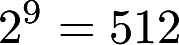
\includegraphics[width=0.64583in,height=0.16667in]{texmath/78dfcc5Cdpi7B3507D25E93D512},因此地址线为9位,再加上一根读控制线和一根写控制线(可能有些书上的答案还会有电源线、地线等,不要想太多,只算读、写线即可),一共是8+9+2=19,故选D。
\end{solution}
